\section{Top Level Design}

\usetikzlibrary{arrows.meta,shapes.geometric,positioning,calc}

\subsection{Overall Block Diagram}

\begin{figure}[H]
\centering
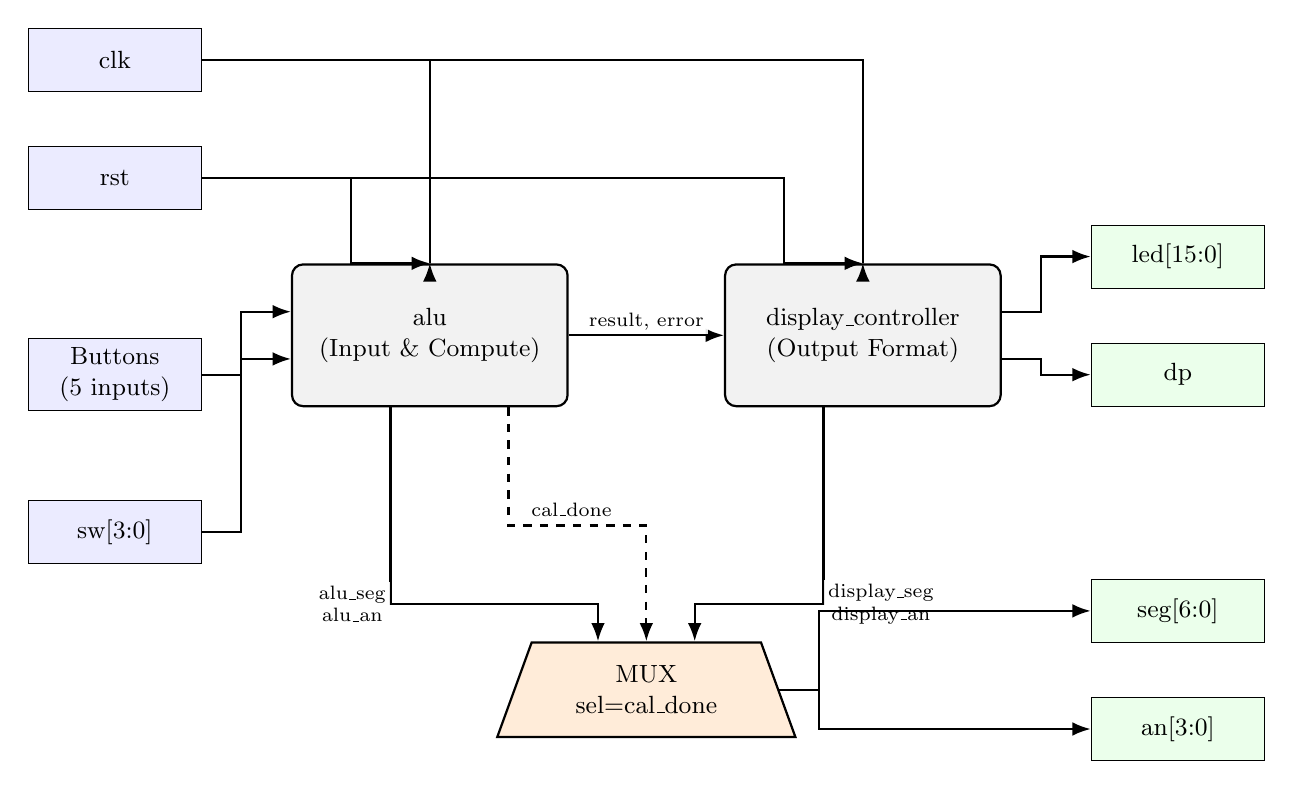
\begin{tikzpicture}[
  font=\small,
  % Node Styles
  block/.style={draw, rounded corners, thick, align=center, minimum height=1.8cm, minimum width=3.5cm, fill=gray!10},
  io_input/.style={draw, rectangle, align=center, minimum height=0.8cm, minimum width=2.2cm, fill=blue!8},
  io_output/.style={draw, rectangle, align=center, minimum height=0.8cm, minimum width=2.2cm, fill=green!8},
  mux/.style={draw, thick, trapezium, trapezium angle=70, minimum width=2.5cm, minimum height=1.2cm, fill=orange!15, align=center},
  % Line Styles
  sig_line/.style={-Latex, thick, black},
  ctrl_line/.style={-Latex, dashed, thick, black},
  % Label Styles
  lbl/.style={font=\scriptsize, align=center, fill=white, inner sep=1.5pt, text opacity=1, fill opacity=0.9}
]

% ================= NODES =================

% --- Inputs (Left Column) ---
\node[io_input] (clk)   at (-6, 3.5) {clk};
\node[io_input] (rst)   at (-6, 2.0) {rst};
\node[io_input] (btns)  at (-6, -0.5) {Buttons\\(5 inputs)};
\node[io_input] (sw)    at (-6, -2.5) {sw[3:0]};

% --- Core Processing (Center) ---
\node[block] (alu)  at (-2, 0) {alu\\(Input \& Compute)};
\node[block] (disp) at (3.5, 0) {display\_controller\\(Output Format)};

% --- MUX (Bottom Center) ---
\node[mux] (mux) at (0.75, -4.5) {MUX\\sel=cal\_done};

% --- Outputs (Right Column) ---
\node[io_output] (led) at (7.5, 1.0) {led[15:0]};
\node[io_output] (dp)  at (7.5, -0.5) {dp};
\node[io_output] (seg) at (7.5, -3.5) {seg[6:0]};
\node[io_output] (an)  at (7.5, -5.0) {an[3:0]};

% ================= CONNECTIONS =================

% 1. Global Signals (Routed via Top)
% Clock
\draw[sig_line] (clk) -- ++(4,0) |- (alu.north);
\draw[sig_line] (clk) -- ++(9.5,0) |- (disp.north);
% Reset
\draw[sig_line] (rst) -- ++(3,0) |- (alu.north);
\draw[sig_line] (rst) -- ++(8.5,0) |- (disp.north);

% 2. Data Inputs to ALU (Direct)
\draw[sig_line] (btns.east) -- ++(0.5,0) |- ($(alu.west)+(0,0.3)$);
\draw[sig_line] (sw.east)   -- ++(0.5,0) |- ($(alu.west)+(0,-0.3)$);

% 3. ALU to Display Controller (Direct Horizontal)
\draw[sig_line] (alu.east) -- node[lbl, above] {result, error} (disp.west);

% 4. ALU to MUX (Left Input)
\draw[sig_line] ($(alu.south)+(-0.5,0)$) -- ++(0,-2.5) coordinate(alu_drop) -- (alu_drop -| mux.north west) -- (mux.north west);
\node[lbl, left] at (alu_drop) {alu\_seg\\alu\_an};

% 5. Display to MUX (Right Input)
\draw[sig_line] ($(disp.south)+(-0.5,0)$) -- ++(0,-2.5) coordinate(disp_drop) -- (disp_drop -| mux.north east) -- (mux.north east);
\node[lbl, right] at (disp_drop) {display\_seg\\display\_an};

% 6. Display to Direct Outputs (LED, DP)
\draw[sig_line] ($(disp.east)+(0,0.3)$) -- ++(0.5,0) |- (led.west);
\draw[sig_line] ($(disp.east)+(0,-0.3)$) -- ++(0.5,0) |- (dp.west);

% 7. MUX to Outputs (SEG, AN)
\draw[sig_line] (mux.east) -- ++(0.5,0) |- (seg.west);
\draw[sig_line] (mux.east) -- ++(0.5,0) |- (an.west);

% 8. Control Signal (cal_done)
% Dashed line from ALU to MUX Select
\draw[ctrl_line] ($(alu.south)+(1.0,0)$) -- ++(0,-1.5) coordinate(ctrl_turn) -- (ctrl_turn -| mux.north) -- (mux.north);
\node[lbl] at ($(ctrl_turn)+(0.8,0.2)$) {cal\_done};

\end{tikzpicture}
\caption{Top-level calculator system architecture showing data flow between modules}
\label{fig:top_level_arch}
\end{figure}

\subsection{Data Flow Description}

The system operates in two phases controlled by the \texttt{cal\_done} signal:

\noindent \textbf{Computation Phase} (\texttt{cal\_done = 0}): The ALU processes user inputs (buttons, switches) and displays intermediate steps on the 7-segment display.
    
\noindent \textbf{Display Phase} (\texttt{cal\_done = 1}): The display controller formats the final result and error status, routing output through the MUX to the 7-segment display, while simultaneously driving LED and decimal point indicators.

